\begin{marginfigure}[9cm]	
\margingraphics{figures/1_3_Act2.eps}
\caption{Axes for plotting $y = s(t)$ in Activity~\ref{A:2.1.2}.} \label{fig:2.1.Act2}
\end{marginfigure}

\begin{activity}  \label{A:2.1.2}
A water balloon is tossed vertically in the air from a window.  The balloon's height in feet at time $t$ in seconds after being launched is given by $s(t) = -16t^2 + 16t + 32$. Use this function to respond to each of the following questions.
\ba
	\item Sketch an accurate, labeled graph of $s$ on the axes provided in Figure~\ref{fig:2.1.Act2}.  You should be able to do this without using computing technology.
		
	\item Compute the average rate of change of $s$ on the time interval $[1,2]$.  Include units on your answer and write one sentence to explain the meaning of the value you found.  
	\item Use the limit definition to compute the instantaneous rate of change of $s$ with respect to time, $t$, at the instant $a = 1$.  Show your work using proper notation, include units on your answer, and write one sentence to explain the meaning of the value you found.
	\item On your graph in (a), sketch two lines:  one whose slope represents the average rate of change of $s$ on $[1,2]$, the other whose slope represents the instantaneous rate of change of $s$ at the instant $a=1$.  Label each line clearly.
	\item For what values of $a$ do you expect $s'(a)$ to be positive?  Why?  Answer the same questions when ``positive'' is replaced by ``negative'' and  ``zero.'' 
\ea
\end{activity}
\begin{smallhint}
\ba
	\item Observe that $(t^2 - t - 2) = (t-2)(t+1)$ and that $s(t)$ has its vertex at $t = \frac{1}{2}$.
	\item Recall the formula for average rate of change.
	\item Note that $s(1+h) = -16(1+h)^2 + 16(1+h) + 32$.
	\item Think about a secant line and a tangent line.
	\item A line with positive slope is one that is rising; a line with negative slope is one that is falling.
\ea
\end{smallhint}
\begin{bighint}
\ba
	\item Show that the quadratic function has $t$-intercepts at $(2,0)$ and $(-1,0)$; $s$-intercept $(0,32)$; and vertex at the point where $t = \frac{1}{2}$.
	\item Compute $\frac{s(2)-s(1)}{2-1}$.
	\item Observe that $s(1+h) - s(1) = (-16(1+h)^2 + 16(1+h) + 32) - (-16(1)^2 + 16(1) + 32) = -16 - 32h - 16h^2 + 16 + 16h + 32 - 32$ and combine like terms carefully.
	\item Consider the line through $(1,s(1))$ and $(2,s(2))$, as well as the line through $(1,s(1))$ with slope $s'(1)$.
	\item Observe that whenever the ball is rising, it's position function is rising, and thus the slope of its tangent line at any such point will be positive.
\ea
\end{bighint}
\begin{activitySolution}
\ba
	\item Since $s(t) = -16t^2 + 16t + 32 = -16(t^2 - t - 2) = -16(t-2)(t+1)$, $s$ has $t$-intercepts at $(2,0)$ and $(-1,0)$; the $s$-intercept is clearly $(0,32)$; and the vertex is $(\frac{1}{2},36)$.
	\item Observe that $\frac{s(2)-s(1)}{2-1} = \frac{0 - 32}{1} = -32$ feet per second.  This value represents the average rate at which the ball is falling over the time interval from $t = 1$ to $t = 2$.
	\item We compute $s'(1)$ as follows:
	\begin{eqnarray*}
		s'(1) & = & \lim_{h \to 0} \frac{s(1+h)-s(1)}{h} \\
		       & = & \lim_{h \to 0} \frac{(-16(1+h)^2 + 16(1+h) + 32) - (-16(1)^2 + 16(1) + 32)}{h} \\
		       & = & \lim_{h \to 0} \frac{-16 - 32h - 16h^2 + 16 + 16h + 32 - 32}{h} \\
		       & = & \lim_{h \to 0} \frac{-16h - 16h^2}{h} \\
		       & = & \lim_{h \to 0} (-16-16h) \\
		       & = & -16.
	\end{eqnarray*}  
	\item We plot and label the secant line through $(1,s(1))$ and $(2,s(2))$, as well as the tangent line through $(1,s(1))$ with slope $s'(1)$.

	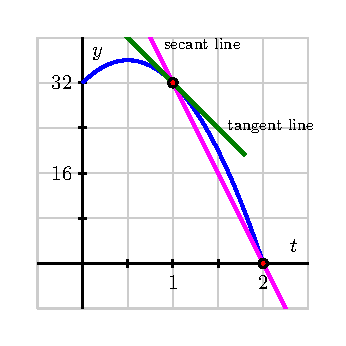
\includegraphics{figures/1_3_Act2Soln.eps}
	
	\item Observe that whenever the ball is rising, it's position function is rising, and thus the slope of its tangent line at any such point will be positive. This means that we should find $s'(a)$ to be positive whenever $0 \le a < \frac{1}{2}$, and similarly $s'(a)$ to be negative whenever $\frac{1}{2} < a < 2$ (which is when the ball is falling).  At the instant $a = \frac{1}{2}$, the ball is at its vertex and is neither rising nor falling, and at that point, $s'(\frac{1}{2}) = 0.$
\ea
\end{activitySolution}
\aftera